\documentclass[a4paper]{extarticle}
\usepackage[utf8]{inputenc}
\usepackage[a4paper, margin=1in]{geometry}

\usepackage{amssymb}
\usepackage{amsmath}
\usepackage{enumitem}
\usepackage{tcolorbox}
\usepackage{fancyhdr}
\usepackage{graphicx}
\usepackage{float}

\setlength{\parindent}{0em}
\setlength{\parskip}{0.4em}

\definecolor{theoremblue}{RGB}{1, 73, 124}
\definecolor{corollaryblue}{RGB}{70, 143, 175}
\definecolor{exampleblue}{RGB}{137, 194, 217}

\newtcolorbox{tbox}{colback=theoremblue!20,colframe=theoremblue,
boxrule=0pt,arc=0pt,boxsep=2pt,left=2pt,right=2pt,leftrule=2pt}

\newtcolorbox{cbox}{colback=corollaryblue!20,colframe=corollaryblue,
boxrule=0pt,arc=0pt,boxsep=2pt,left=2pt,right=2pt,leftrule=2pt}

\newtcolorbox{ebox}{colback=exampleblue!20,colframe=exampleblue,
boxrule=0pt,arc=0pt,boxsep=2pt,left=2pt,right=2pt,leftrule=2pt}

\title{IntroML - Lecture Notes Week 9}
\author{Ruben Schenk, ruben.schenk@inf.ethz.ch}
\date{\today}

\pagestyle{fancy}
\fancyhf{}
\rhead{ruben.schenk@inf.ethz.ch}
\rfoot{Page \thepage}
\lhead{IntroML - Lecture Notes Week 9}

\begin{document}

\maketitle

\section{Unsupervised Learning: Dimension Reduction}

\subsection{Introduction}

The basic challenge is posed as follows: Given a data set $D = \{x_1,..., \, x_n\}$ with $x_i \in \mathbb{R}^d$, obtain an \textbf{embedding} (low-dimensional representation) $z_1,..., \, z_n \in \mathbb{R}^k$ where typically $k << d$.

One might want to do this for several reasons:
\begin{itemize}
    \item Visualization ($k = 1, \, 2, \, 3$)
    \item Regularization (model selection)
    \item Unsupervised feature discovery (i.e. determining features from data)
    \item etc.
\end{itemize}

\textbf{Note:} Our focus is on model-based approaches, i.e.:
\begin{itemize}
    \item Given: Data $D = \{x_1,..., \, x_n\} \subseteq \mathbb{R}^d$
    \item Goal: Obtain a mapping $f : \mathbb{R}^d \to \mathbb{R}^k$ where usually $k << d$
    \item We can distinguish:
    \begin{itemize}
        \item Linear dimension reduction $f(x) = Ax$
        \item Nonlinear dimension reduction (parametric or non-parametric)
    \end{itemize}
\end{itemize}

\subsection{Dimension Reduction}

\textbf{Linear dimension redcution} can be seen as compression. The motivation behind this process is that low-dimensional representation should allow to compress the original data and allow for a accurate reconstruction.

Let us consider a simple example for $k = 1$. Given is a data set $D = \{x_1,..., \, x_n\} \subseteq \mathbb{R}^d$, assumed to be centered, i.e. $\mu = \frac{1}{n} \sum_i x_i = 0$. We want to represent the data as points on a line $x_i \approx z_iw$ with coefficients $w \in \mathbb{R}^d$.

\begin{figure}[H]
    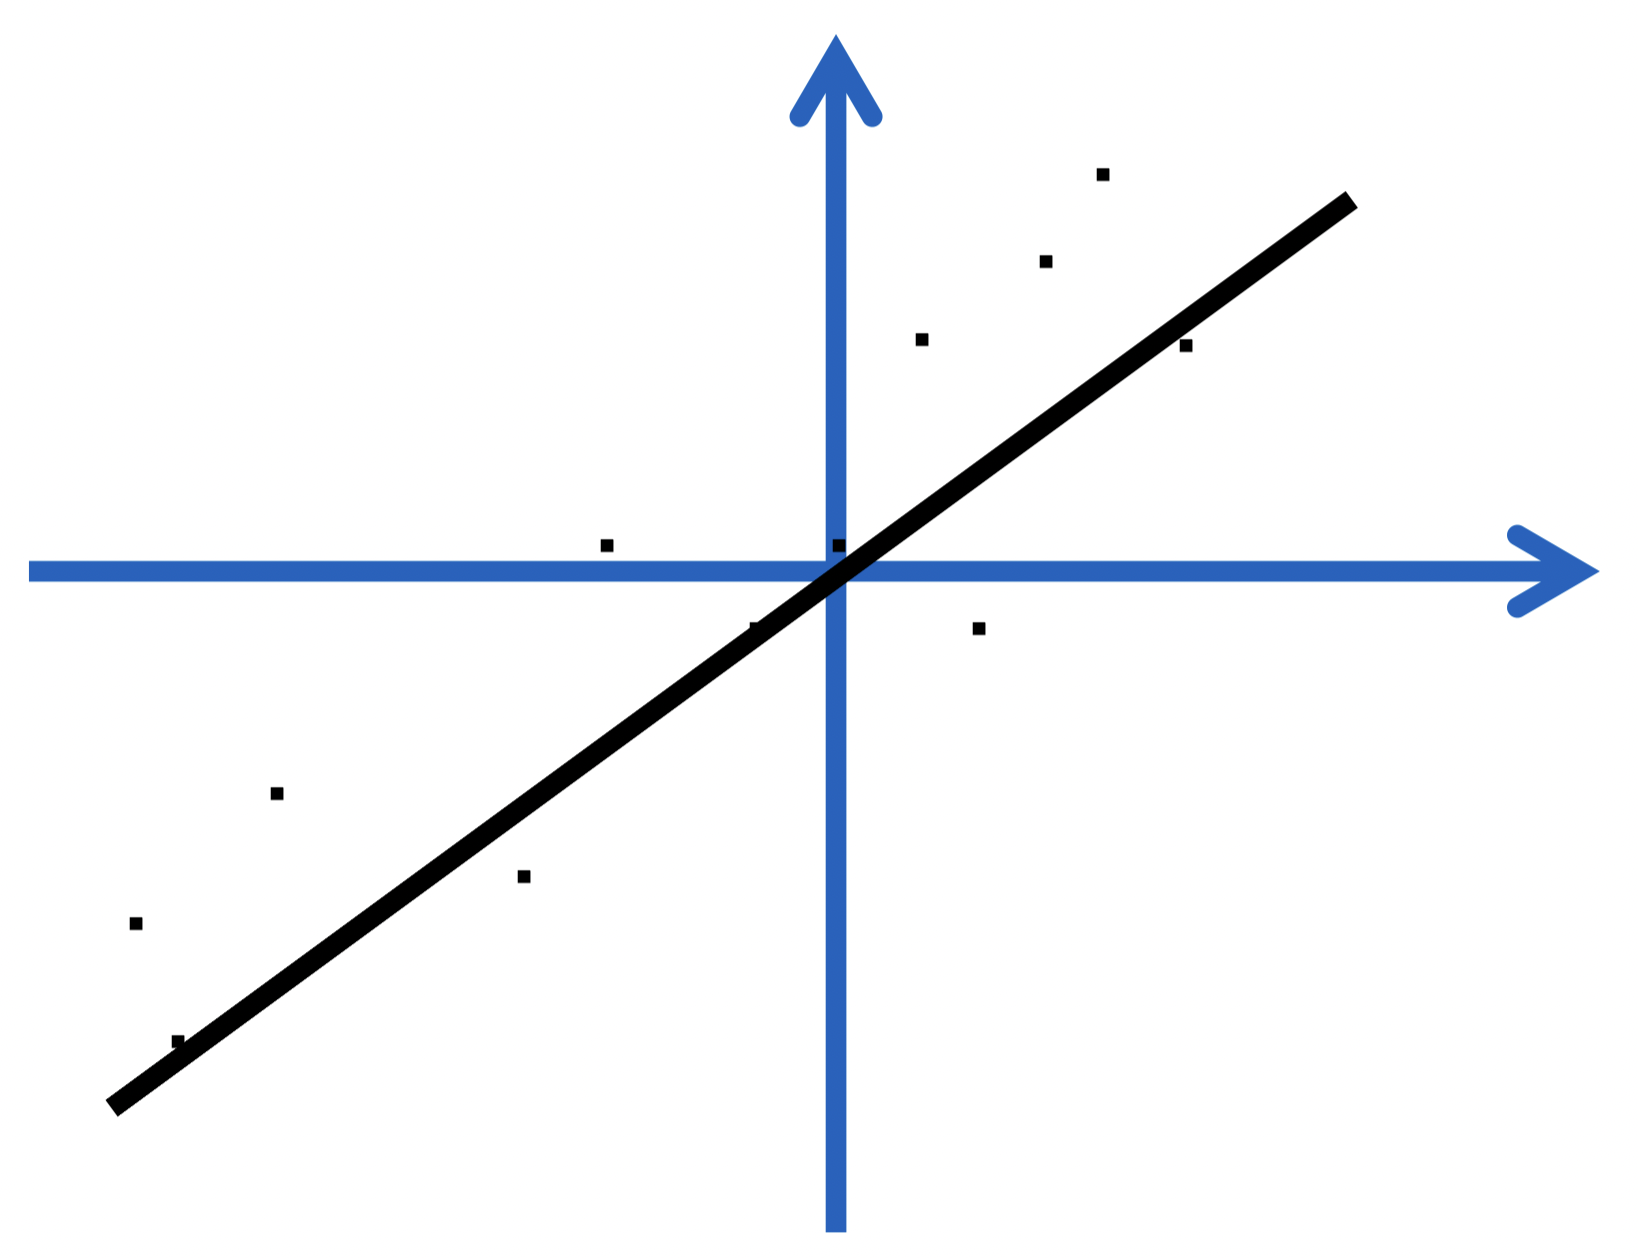
\includegraphics[width=5cm]{../images/IntroML_Fig9-1}
    \centering
\end{figure}

In other words, we want $x_i \approx z_iw$ minimizing $||z_iw - x_i||_2^2$. To ensure the uniqueness of the solution, we normalize $w$, i.e. $||w||_2 = 1$. We want to optimize jointly over $w, \, z_1, \, z_2,...$:

\[
    (w^*, \, z^*) = \arg \min_{||w||_2 = 1, \, z} \sum_{i = 1}^n ||z_iw - x_i||_2^2.
\]

In our $k = 1$ case, the optimal $z$ is given by:

\[
    z_i^* = w^Tx_i
\]

Thus, we effectively solve a \textit{regression} problem, interpreting $x$ as features and $z$ as labels. Since for any fixed $||w||_2 = 1$, it holds that $z_i^* = w^Tx_i$. Therefore, we only need:

\[
    w^* = \arg \min_{||w||_2 = 1} \sum_{i = 1}^n ||ww^Tx_i - x_i||_2^2,
\]
which is equivalent to
\[
    w^* = \arg \min_{||w||_2 = 1} \sum_{i = 1}^n (w^Tx_i)^2,
\]
which is furthermore equivalent to
\[
    w^* = \arg \max_{||w||_2 = 1} w^T\Sigma w,
\]
where $\Sigma = \frac{1}{n}\sum_{i = 1}^n x_ix_i^T$ is the \textit{empirical covariance,} assuming the data is centered (i.e. $\mu = \frac{1}{n} \sum_i x_i = 0$).

Finally, the optimal solution to $w^* = \arg \max_{||w||_2 = 1} w^T\Sigma w$ is given by the \textbf{principal eigenvector} of $\Sigma$, i.e. $w = v_1$ where, for $\lambda_1 \geq \cdots \geq \lambda_d \geq 0$,

\[
    \Sigma = \sum_{i = 1}^d \lambda_i v_i v_i^T.
\]

But what if $k > 1$? Suppose we wish to project more than one dimension. Thus we want:

\[
    (W, \, z_1,..., \, z_n) = \arg \min_{W^TW = I_k, \, z} \sum_{i = 1}^n ||Wz_i - x_i||_2^2,
\]

where $W \in \mathbb{R}^{d \times k}$ is \textit{orthogonal,} and $z_1,..., \, z_n \in \mathbb{R}^k$. This is called the \textit{principal component analysis} problem and its solution can be obtained in closed form even for $k > 1$.

\subsection{Principle Component Analysis (PCA)}

The \textbf{Principal Component Analysis (PCA)} problem is as follows:

Given centered data $D = \{x_1,..., \, x_n\} \subseteq \mathbb{R}^d$ with $\mu = \frac{1}{n} \sum_i x_i = 0$ and $\Sigma = \frac{1}{n} \sum_{i = 1}^n x_ix_i^T$, the solution to the PCA problem
\[
    (W, \, z_1,..., \, z_n) = \arg \min_{W^TW = I_k, \, z} \sum_{i = 1}^n ||Wz_i - x_i||_2^2,
\]
where $1 \leq k \leq d, \, W \in \mathbb{R}^{d \times k}$ is orthogonal and $z_1,..., \, z_n \in \mathbb{R}^k$, is given by

\[
    W = (v_1 \, | \, \cdots \, | \, v_k) \text{ and } z_i = W^Tx_i.
\]
Hereby: $\Sigma = \sum_{i = 1}^d \lambda_iv_iv_i^T$ and $\lambda_1 \geq \cdots \geq \lambda_d$.

The linear mapping $f(x) = W^Tx$ obtained from PCA \textit{projects} vectors $x \in \mathbb{R}^d$ into a $k$-dimensional subspace. This projection is chosen to \textit{minimize the reconstruction error} (measured in the Euclidean norm).

One might remember that we can obtain PCA through the \textit{Singular-Value Decomposition (SVD).} We recall that any $X \in \mathbb{R}^{n \times d}$ can be represented as

\[
    X = USV^T,
\]

where $U \in \mathbb{R}^{n \times n}$ and $V \in \mathbb{R}^{d \times d}$ are orthogonal, and $S \in \mathbb{R}^{n \times d}$ is diagonal (w.l.o.g. in decreasing order). Its entries are called \textit{singular values.} The top $k$ principal components are exactly the first $k$ columns of $V$:

\[
    n\Sigma = X^TX = VS^TU^TUSV^T = VS^TSV^T = VDV^T.
\]

Finally, we can compare PCA and k-means:

\textbf{PCA-Problem:}
\[
    (W, \, z_1,..., \, z_n) = \arg \min_{W^TW = I_k, \, z} \sum_{i = 1}^n ||Wz_i - x_i||_2^2,
\]
where $W \in \mathbb{R}^{d \times k}$ is \textit{orthogonal,} and $z_1,..., \, z_n \in \mathbb{R}^k$.

\textbf{k-means problem (equivalent formulation):}
\[
    (W, \, z_1,..., \, z_n) = \arg \min_{W, \, z} \sum_{i = 1}^n ||Wz_i - x_i||_2^2,
\]
where $W \in \mathbb{R}^{d \times k}$ is \textit{arbitrary,} and $z_1,..., \, z_n \in E_k$ for $E_k = \{e_1,..., \, e_k\}$ are all unit vectors.

In summary:
\begin{itemize}
    \item We can think of PCA and k-means as options to solve a similar unsupervised learning problem, with different constraints.
    \item Both aim to compress the data with maximum fidelity under constraints on the model complexity.
    \item This insight gives rise to a much broader class of techniques.
\end{itemize}

\subsection{Kernel PCA}

\subsection{Neural Network Autoencoders}

\end{document}